\documentclass[a4paper, 12pt, brazilian]{article}
\usepackage{config}

\usepackage[utf8]{inputenc}
\usepackage{amsmath, amssymb, amsfonts}
\usepackage[T1]{fontenc}

\usepackage{xcolor}

\usepackage{graphicx}
\usepackage[brazilian]{babel}
\usepackage{hyperref}
\usepackage{cleveref}
\usepackage{float}
\usepackage[top=1cm,right=3cm,bottom=2cm,left=3cm]{geometry}
\usepackage{bm}
\usepackage{xwatermark}
\newwatermark[
	allpages, 
	scale=4, 
	color=magenta!7!green!15, 
	angle=60,
	xpos=-10,
	ypos=10
]{Resumo}

\newcommand{\bfit}[1]{\textit{\textbf{#1}}}
\newcommand{\vect}{\bm{P}_{1}\bm{P}_{0}}
\newcommand{\proj}[2]{\textrm{proj}_{\bfit{#1}}\bfit{#2}}

\title{Reflexões de GA}
\author{Renan Guedes}

\begin{document}
	\maketitle
	\section{Projeção de vetores}
	\begin{figure}[H]
		\centering
		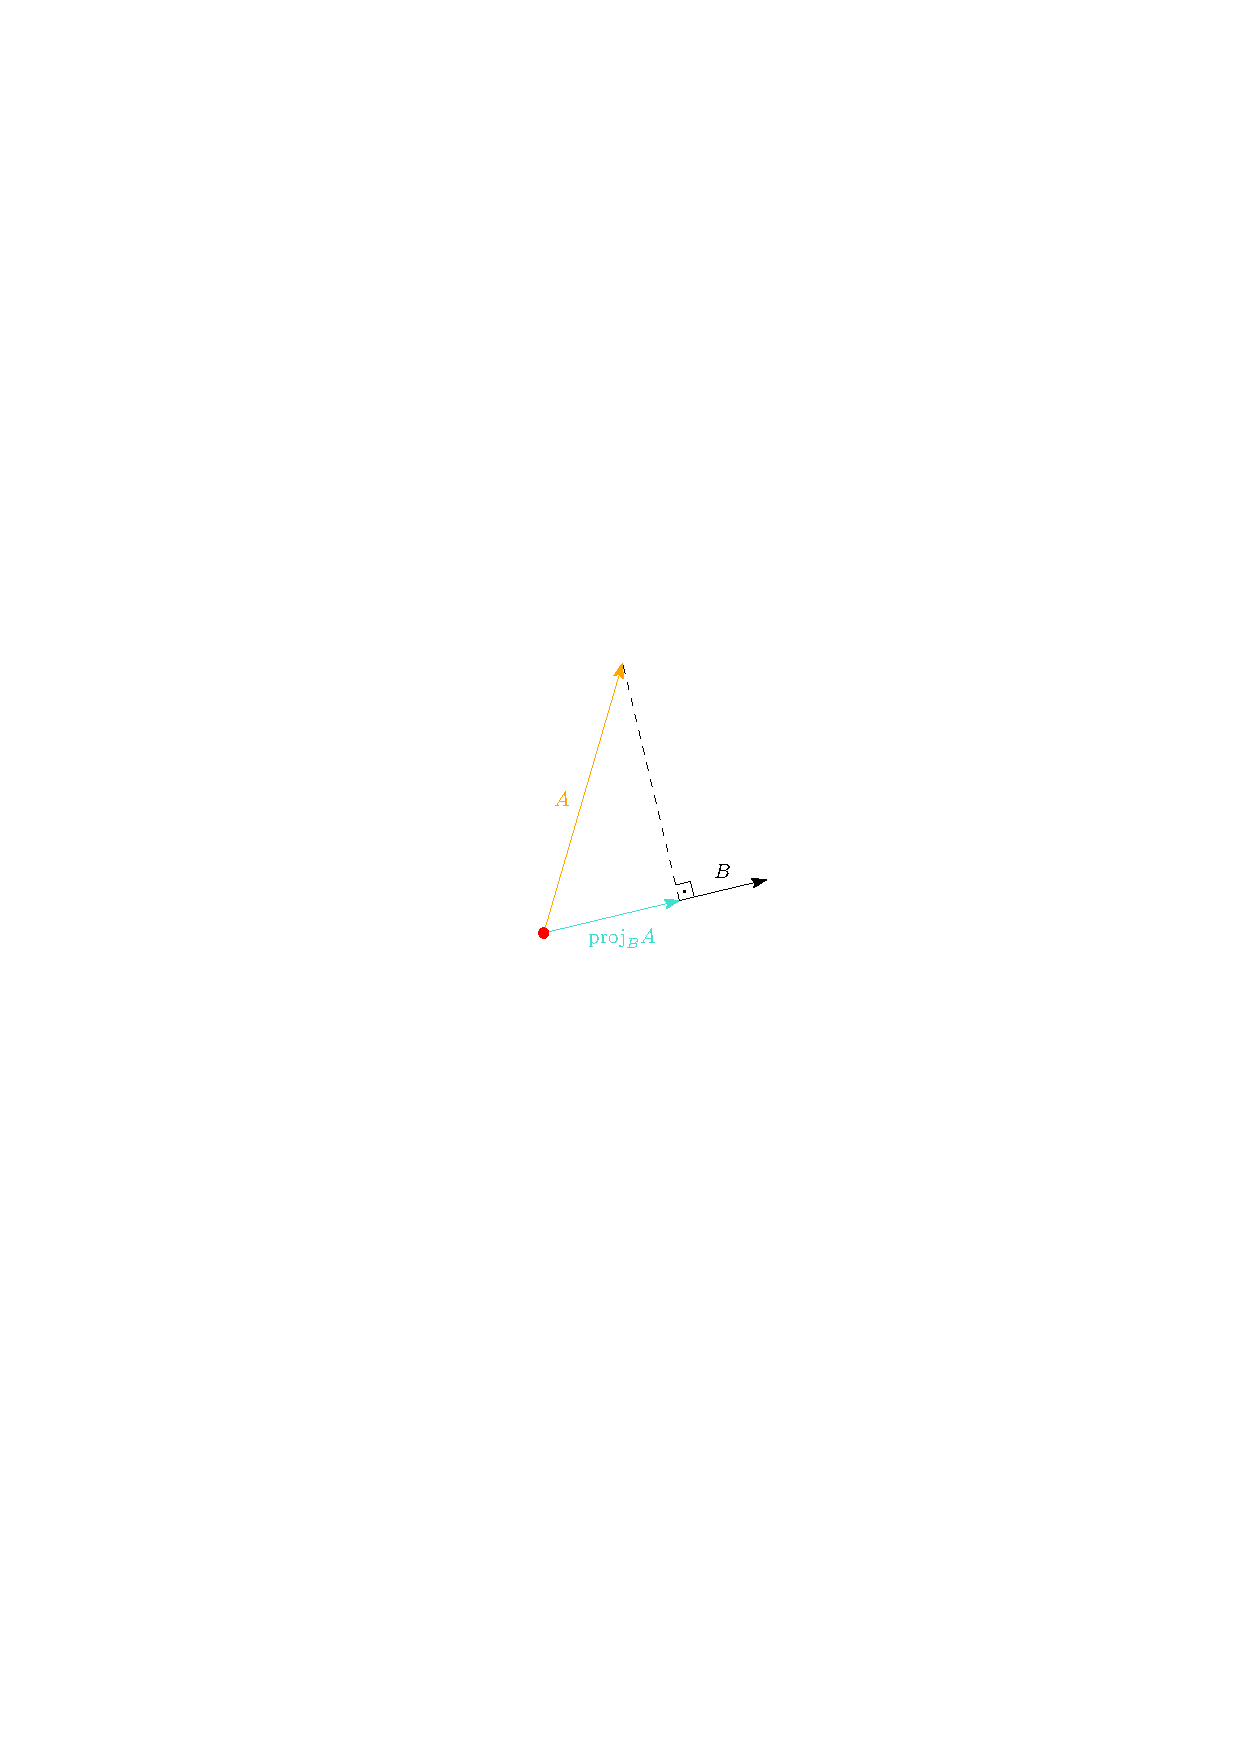
\includegraphics[scale=1.1]{images/proj}
	\end{figure}
	A figura acima ilustra a projeção ortogonal que o vetor $\bm{A}$ faz sobre $\bm{B}$. Essa projeção existe quando sua subtração de $\bm{A}$ gera um vetor ortogonal a \bm{B}. Para chegar na relação que expressa essa medida em termos dos vetores $\bm{A}$ e $\bm{B}$ vamos consideram que $\bm{V}_{1}$ é igual a projeção de $\bm{A}$ sobre $\bm{B}$ e $\bm{V}_{2}$ é o vetor ortogonal a $\bm{B}$ dado por $\bm{A}-\proj{B}{A}$, então
	$$
	\begin{cases}
		\bm{V}_{1}=\proj{B}{A}\\
		\bm{V}_{2}=\bm{A}-\proj{B}{A}
	\end{cases}
	$$	
	Como \bm{V}$_{1}$ é um múltiplo escalar de \bm{B} (vetores paralelos), então é possível escrever \bm{V}$_{1}$ em termos de \bm{B}, como
	\begin{equation}
		\label{eq:first}
		\bm{V}_{1}=\alpha\bm{B}
	\end{equation}
	Ao fazer o produto ponto entre \bm{B} e \bm{V}$_{2}$, temos
	\begin{eqnarray}
		\bm{B}\cdot\bm{V}_{2}&=&\bm{B}\cdot(\bm{A}-\alpha\bm{B})\\
	\end{eqnarray}
	sendo $\bm{B}\bm{B}=||\bm{B}||\,||\bm{B}||\cos 0^{\circ}=||\bm{B}||^{2}$ e $\bm{B}\cdot\bm{V}_{2}=0$ (perpendiculares), vem
	\begin{equation}
		0=\bm{A}\bm{B}-\alpha ||\bm{B}||^{2}
	\end{equation}
	logo $\alpha$ será
	\begin{equation}
		\label{eq:alpha}
		\alpha=\dfrac{\bm{A}\bm{B}}{||\bm{B}||^{2}}
	\end{equation}
	retornando na \cref{eq:first} e substituindo o que foi encontrado em \cref{eq:alpha}, obtemos
	\begin{equation}
		\bm{V}_{1}=\proj{B}{A}=\left(\dfrac{\bm{A}\bm{B}}{||\bm{B}||^{2}}\right)\bm{B}
	\end{equation}
	\section{Distância de um ponto a uma reta}
	\begin{figure}[H]
		\centering
		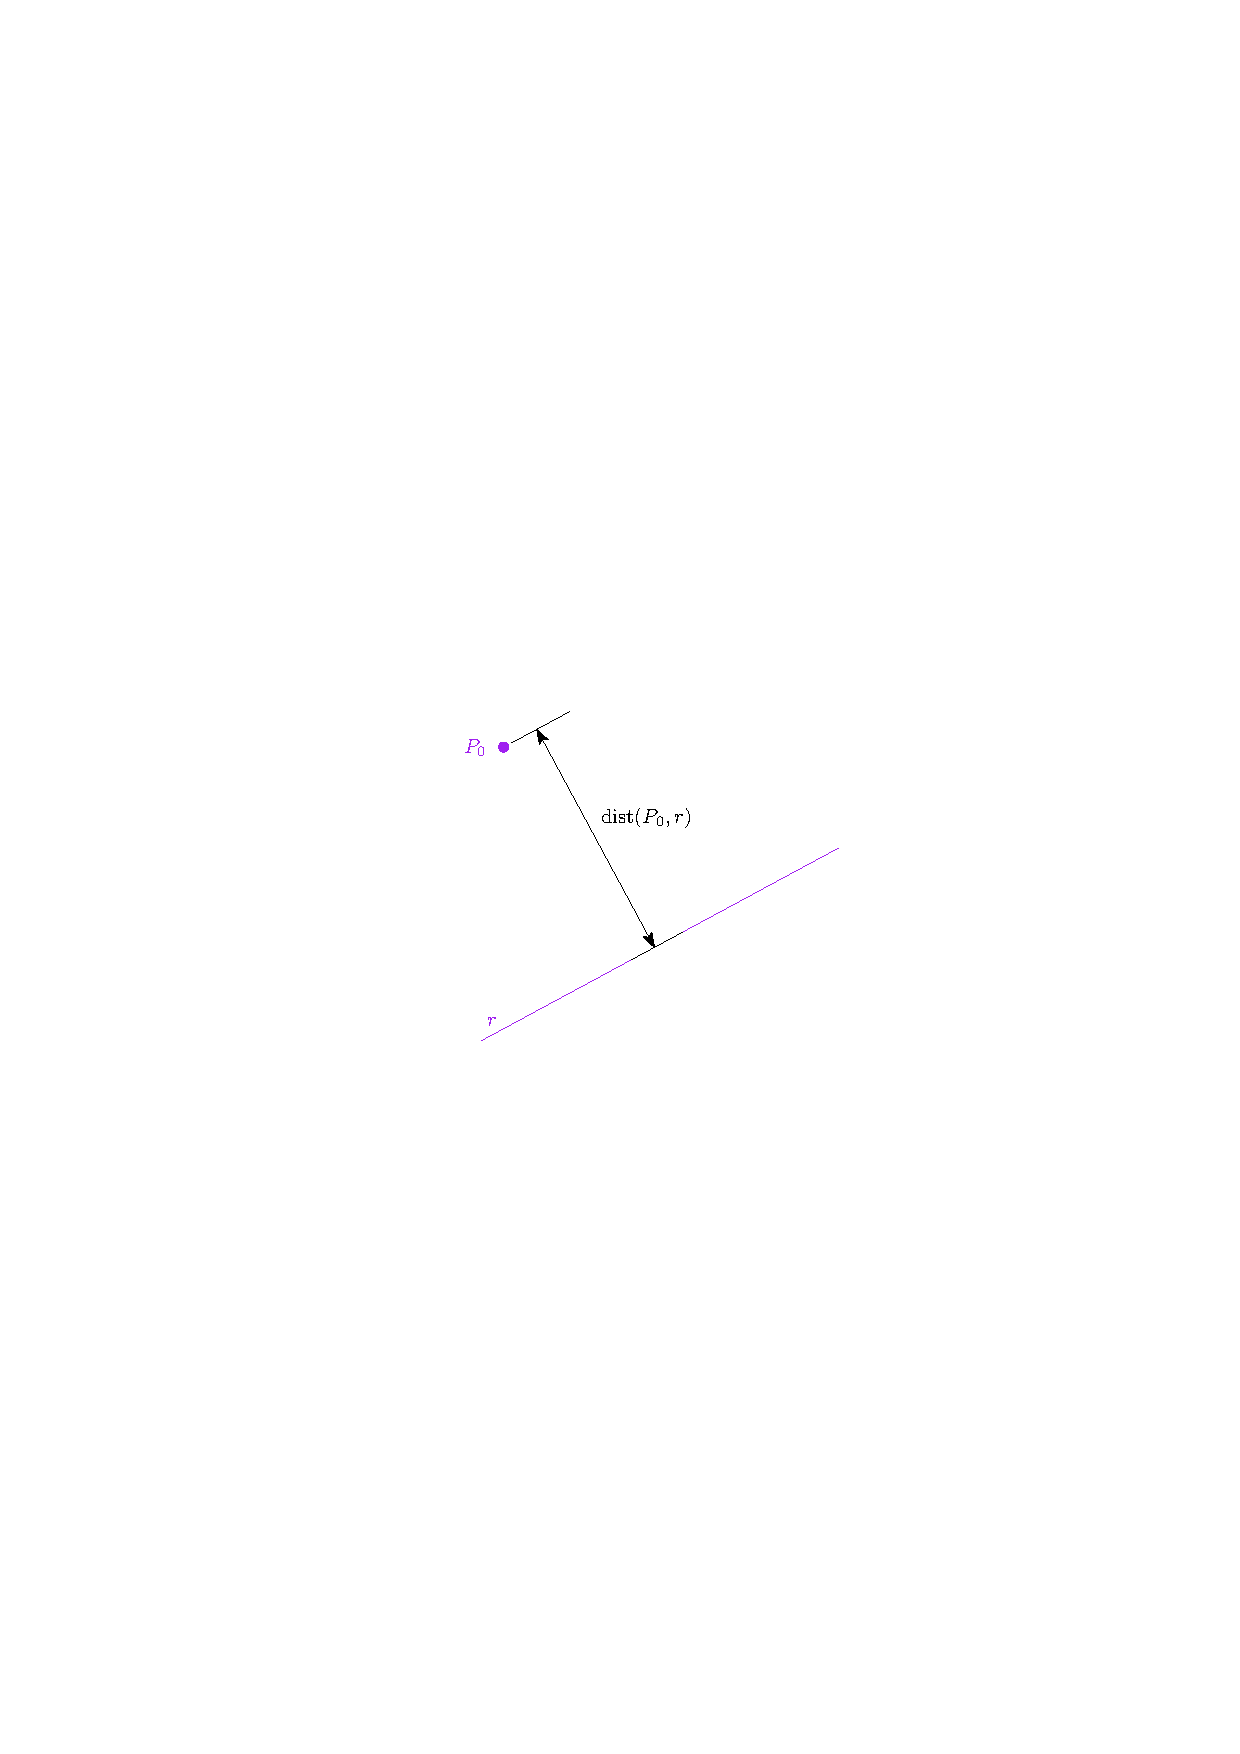
\includegraphics[scale=1.1]{images/dist}
		\label{fig:dist}
	\end{figure}
	Visando dar uma abordagem vetorial ao problema, vamos redesenhar a figura
	\begin{figure}[H]
		\centering
		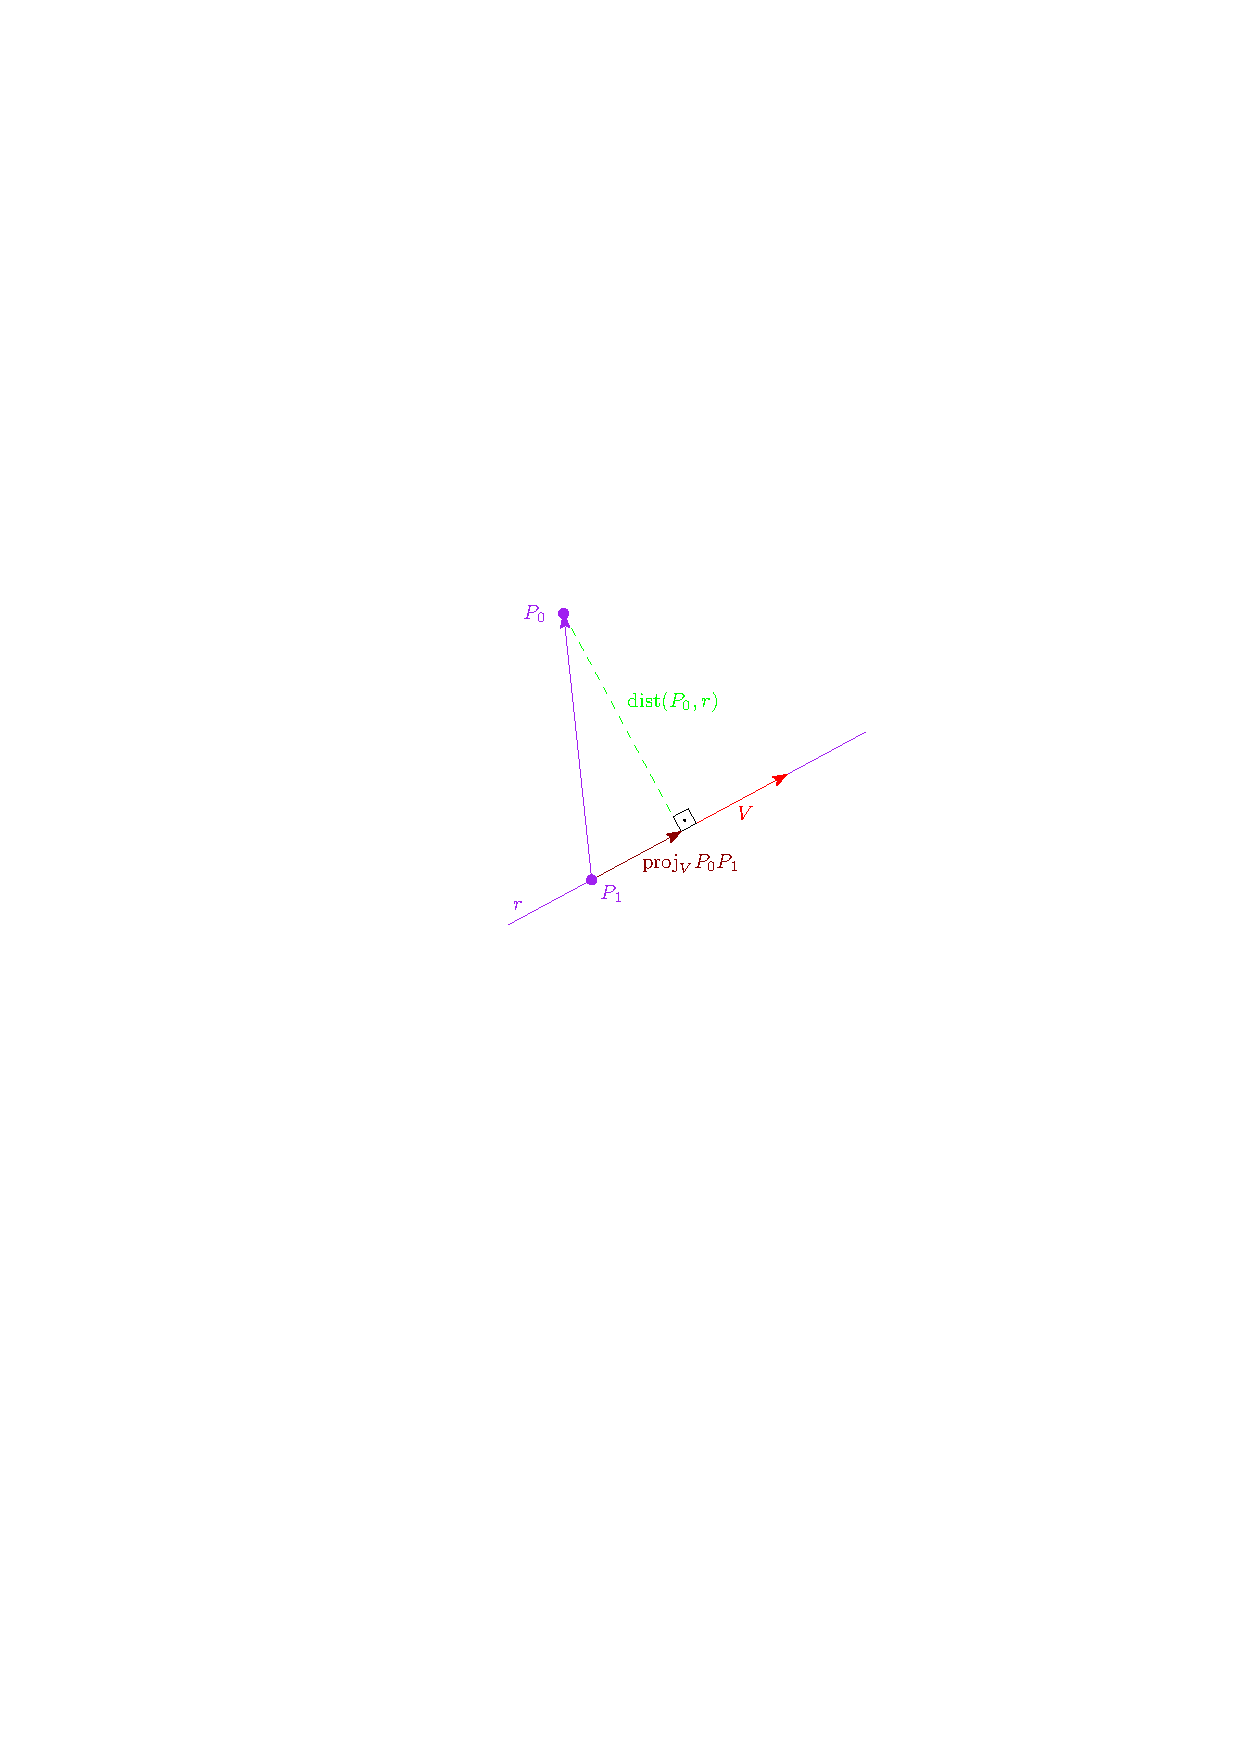
\includegraphics[scale=1.1]{images/dist_n}
		\label{fig:distn}
	\end{figure}
	\noindent aplicando o teorema de Pitágoras, vem
	\begin{eqnarray}
		(\textrm{dist}(P_{0},r))^{2}&=&||\vect||^{2}-||\textrm{proj}_{\bm{V}}\vect||^{2}\\
		&=&||\vect||^{2}-\left|\!\left|\left(\dfrac{\vect\cdot\bm{V}}{||\bm{V}||^{2}}\right)\bm{V}\right|\!\right|^{2}\\
		&=&||\vect||^{2}-\dfrac{(\vect\cdot\bm{V})^{2}}{||\bm{V}||^{2}}
	\end{eqnarray}
	como $\vect\cdot\bm{V}=||\vect||\,||\bm{V}||\cos\theta$, então
	\begin{eqnarray}
		&=&\dfrac{||\vect||^{2}\,||\bm{V}||^{2}}{||\bm{V}||^{2}}-\dfrac{||\vect||^{2}\,||\bm{V}||^{2}\cos^{2}\theta}{||\bm{V}||^{2}}
	\end{eqnarray}
	colocando em evidência
	\begin{eqnarray}
		&=&\dfrac{||\vect||^{2}\,||\bm{V}||^{2}(1-\cos^{2}\theta)}{||\bm{V}||^{2}}
	\end{eqnarray}
	usando a relação fundamental da trigonometria ao considerar que $\sin^{2}\theta=1-\cos^{2}\theta$, substituindo
	\begin{eqnarray}
		\label{eq:cross}
		&=&\dfrac{||\vect||^{2}\,||\bm{V}||^{2}\sin^{2}\theta}{||\bm{V}||^{2}}
	\end{eqnarray}
	dessa forma, o numerador da \cref{eq:cross} é o produto vetorial entre $\vect$ e $\bm{V}$, temos que a distância de $\bm{P}_{0}$ a \textit{r} ao quadrado assumirá
	\begin{equation}
		(\textrm{dist}(P_{0},r))^{2}=\left(\dfrac{\vect\times\bm{V}}{||\bm{V}||}\right)^{\!\!2}
	\end{equation}
	após elevar ambos os lados a $1/2$, temos que a distância será
	\begin{equation}
		\textrm{dist}(P_{0},r)=\dfrac{\vect\times\bm{V}}{||\bm{V}||}
	\end{equation}
	\section{Produto Vetorial}
	Foi visto na seção anterior que para o cálculo da distância entre um ponto e uma reta é requerido o uso do produto vetorial 
	entre um vetor que ligue um ponto de $r$ ao ponto que se deseja saber a distância. Todavia, um questionamento que pode surgir seria o motivo do produto vetorial ser constante, tendo em vista que o ponto $P_{1}$ de $r$ ao ser escolhido de forma arbitrária gera um $\vect$ distinto em cada situação.\vspace{.25cm}
	Uma justificativa que pode ser aplicada é lembrar que o produto vetorial entre dois vetores produz um vetor ortogonal aos dois primeiros com a magnitude dada pela área do paralelogramo formado entre eles. Com base nisso, o que torna o produto cruz $\vect\times\bm{V}$ constante é o fato de que a distância entre a reta $r$ e o ponto $P_{0}$ é constante independente do vetor diretor de $r$ ou do vetor que liga $P_{1}$ a $P_{0}$. Logo, por mais que o vetor $\vect$ não seja ortogonal a $r$ há uma compensação entre o valor do seno de $\theta$ e o comprimento de $\vect$, gerando sempre a mesma projeção da distância. Imaginando que o comprimento de $\vect$ aumente por conta de um ponto $P_{1}\in r$ muito afastado de $P_{0}$, nesse caso, $\theta$ irá diminuir e junto dele o seu seno. Entretanto, caso a distância entre $P_{1}$ e $P_{0}$ diminua, $\theta$ aumentará até que seu seno se torne 1, o que caracteriza a menor distância em linha reta, porém, em ambos os casos, ao considerar que $\bm{V}$ é o mesmo, então $||\vect||\sin\theta$ não mudará.
	
	\begin{figure}[H]
		\centering
		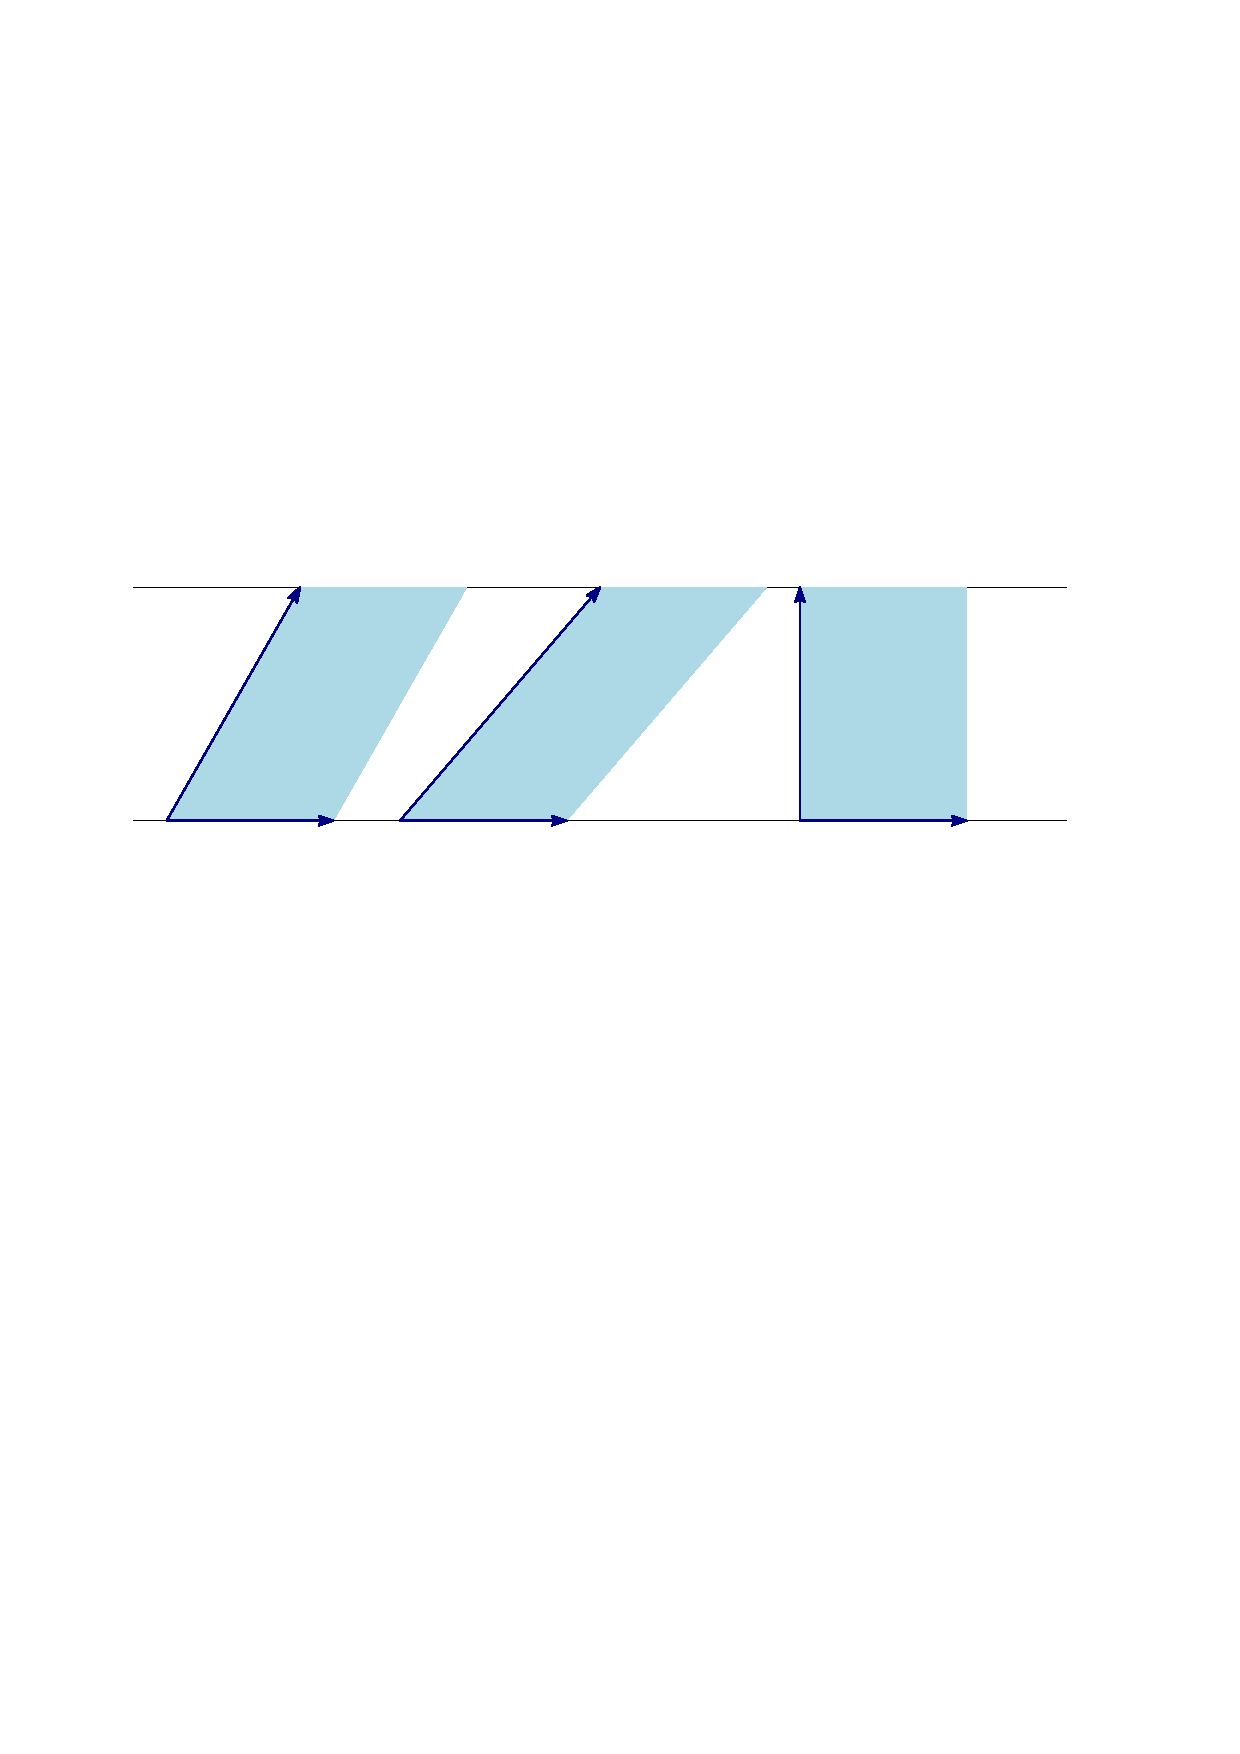
\includegraphics[width=.95\linewidth]{images/area}
		\label{fig:area}
	\end{figure}
	\begin{figure}[H]
		\centering
		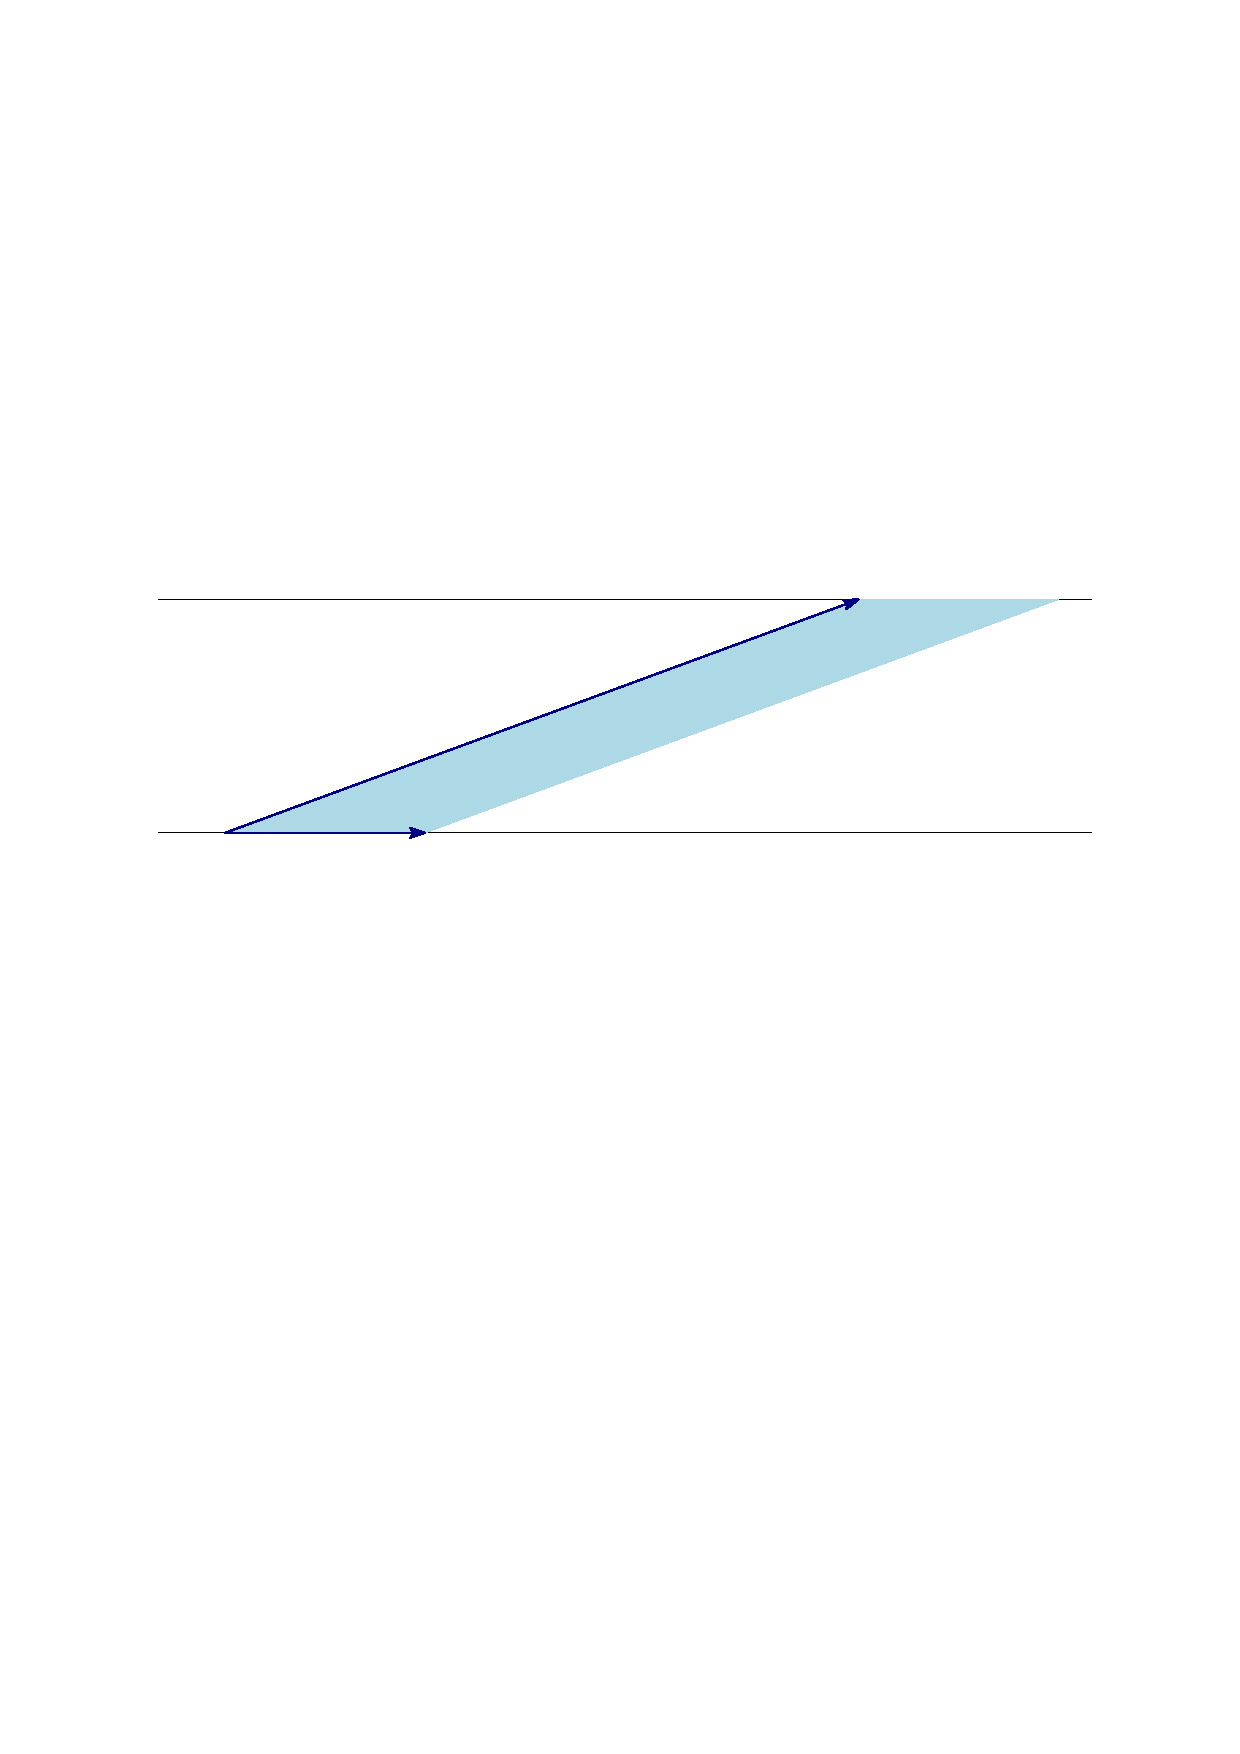
\includegraphics[width=.95\linewidth]{images/area_n}
		\label{fig:arean}
	\end{figure}
	
	
	
\end{document}